\documentclass[a4paper,12pt]{article}

%%% Работа с русским языком
\usepackage{cmap}					% поиск в PDF
\usepackage{mathtext} 				% русские буквы в формулах
\usepackage[T2A]{fontenc}			% кодировка
\usepackage[utf8]{inputenc}			% кодировка исходного текста
\usepackage[english,russian]{babel}	% локализация и переносы
\usepackage{xcolor}
\usepackage{hyperref}
 % Цвета для гиперссылок
\definecolor{linkcolor}{HTML}{799B03} % цвет ссылок
\definecolor{urlcolor}{HTML}{799B03} % цвет гиперссылок

\hypersetup{pdfstartview=FitH,  linkcolor=linkcolor,urlcolor=urlcolor, colorlinks=true}

%%% Дополнительная работа с математикой
\usepackage{amsfonts,amssymb,amsthm,mathtools} % AMS
\usepackage{amsmath}
\usepackage{icomma} % "Умная" запятая: $0,2$ --- число, $0, 2$ --- перечисление

%% Номера формул
%\mathtoolsset{showonlyrefs=true} % Показывать номера только у тех формул, на которые есть \eqref{} в тексте.

%% Шрифты
\usepackage{euscript}	 % Шрифт Евклид
\usepackage{mathrsfs} % Красивый матшрифт

%% Свои команды
\DeclareMathOperator{\sgn}{\mathop{sgn}}

%% Перенос знаков в формулах (по Львовскому)
\newcommand*{\hm}[1]{#1\nobreak\discretionary{}
{\hbox{$\mathsurround=0pt #1$}}{}}
% графика
\usepackage{graphicx}
\graphicspath{{pictures/}}
\DeclareGraphicsExtensions{.pdf,.png,.jpg}
\author{Бурмашев Григорий, БПМИ-208}
\title{Язык SQL, дз -- 5}
\date{\today}
\begin{document}
\maketitle
\clearpage
\section*{Номер 2}
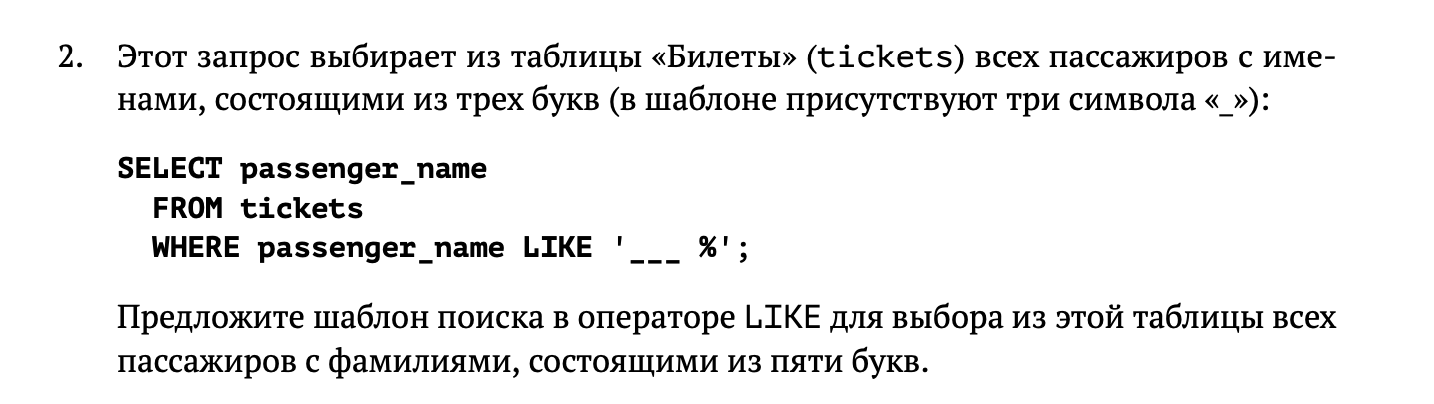
\includegraphics[scale=0.6]{t2.png}
\\\\
\begin{center}
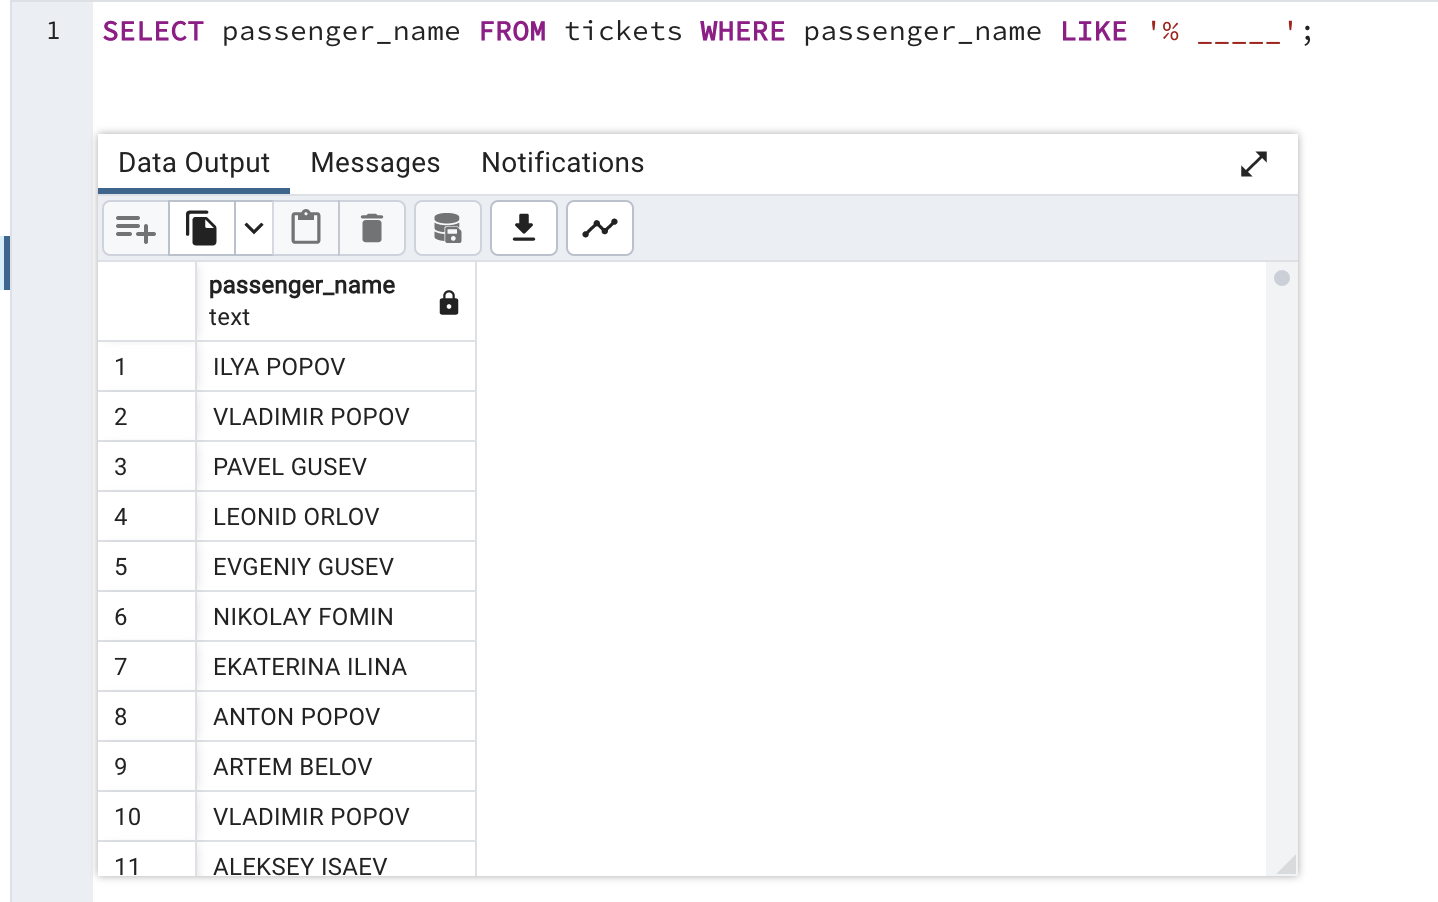
\includegraphics[scale=0.5]{21.png}
\end{center}
\clearpage
\section*{Номер 7}
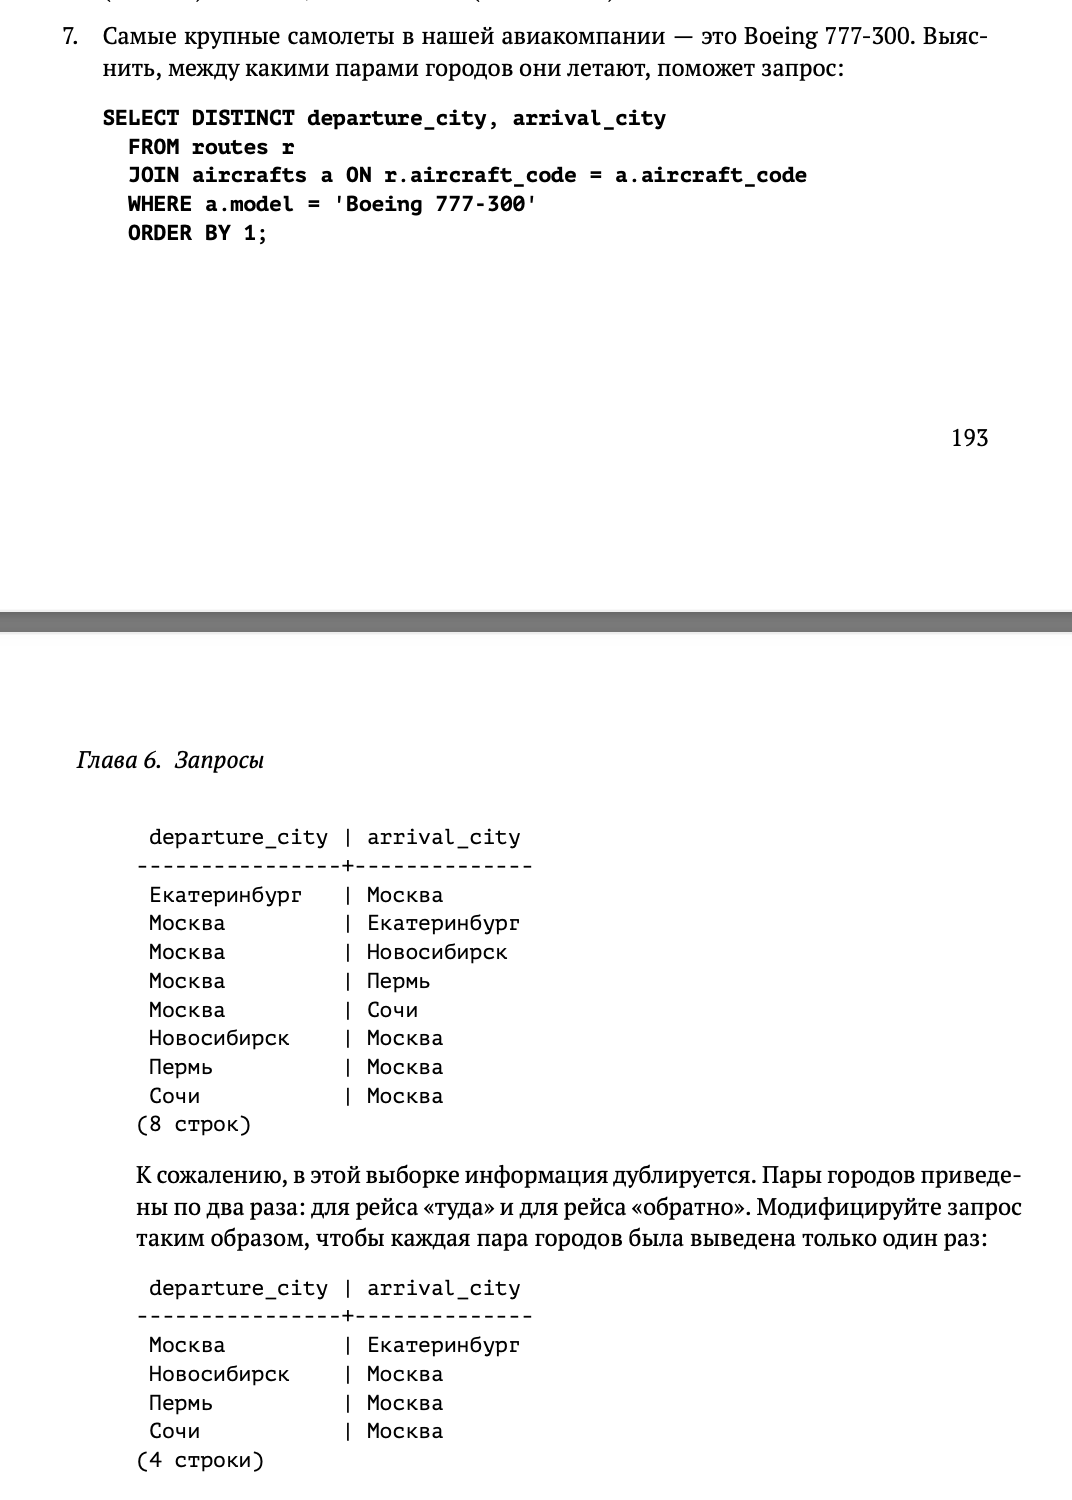
\includegraphics[scale=0.6]{t7.png}
\begin{center}
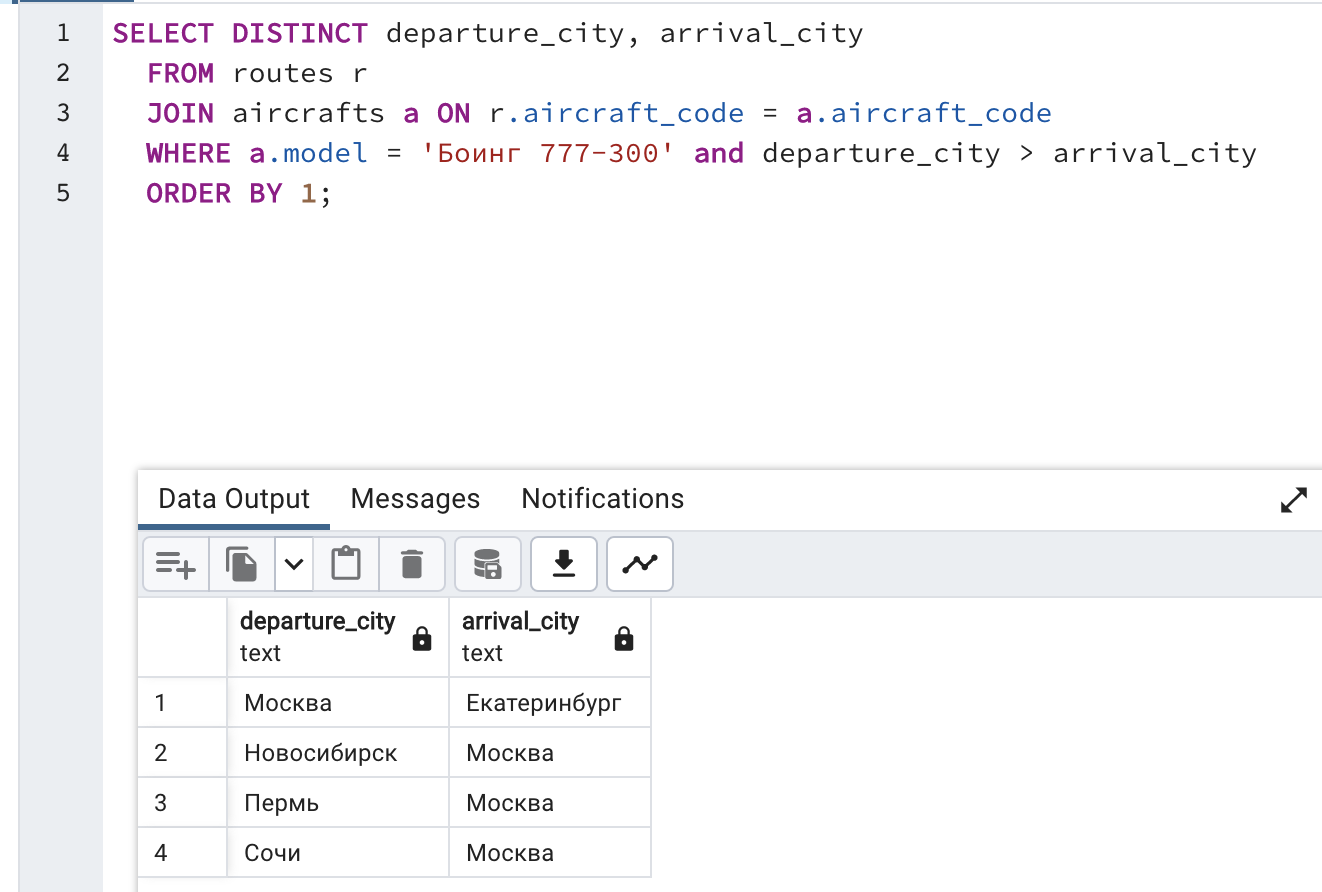
\includegraphics[scale=0.5]{71.png}
\end{center}
В моей бд почему-то aircrafts.model на русском, но это не влияет на решение
\clearpage
\section*{Номер 9}
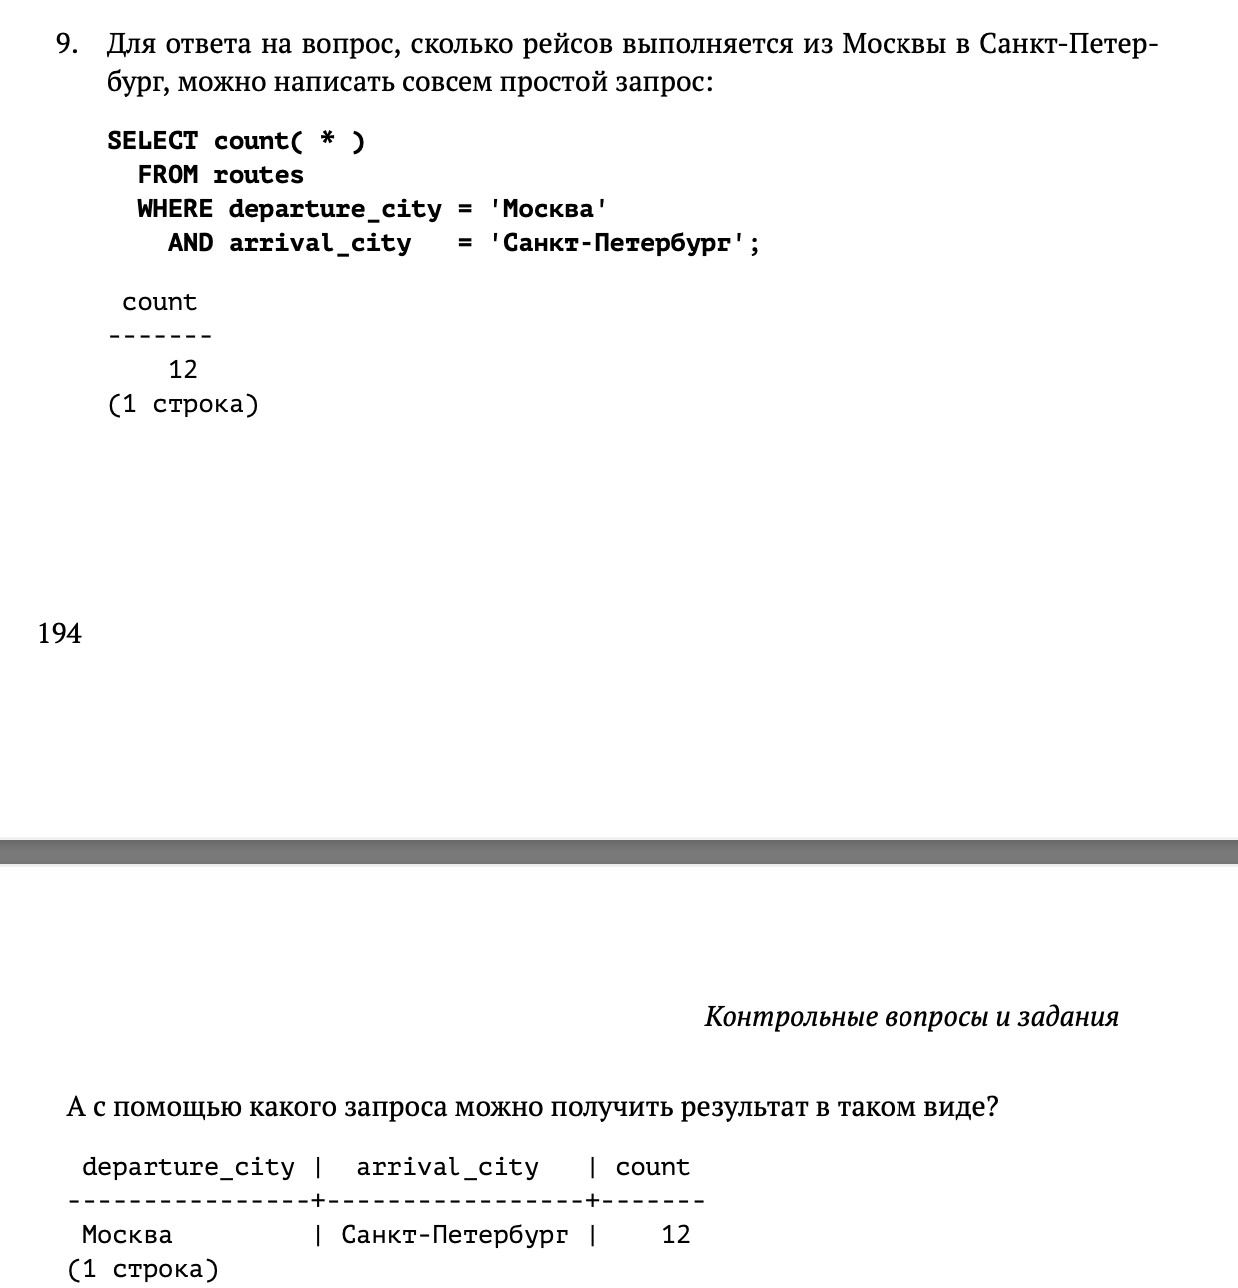
\includegraphics[scale=0.6]{t9.png}
\\\\
\begin{center}

\includegraphics[scale=0.5]{91.png}
\end{center}
\clearpage
\section*{Номер 13}
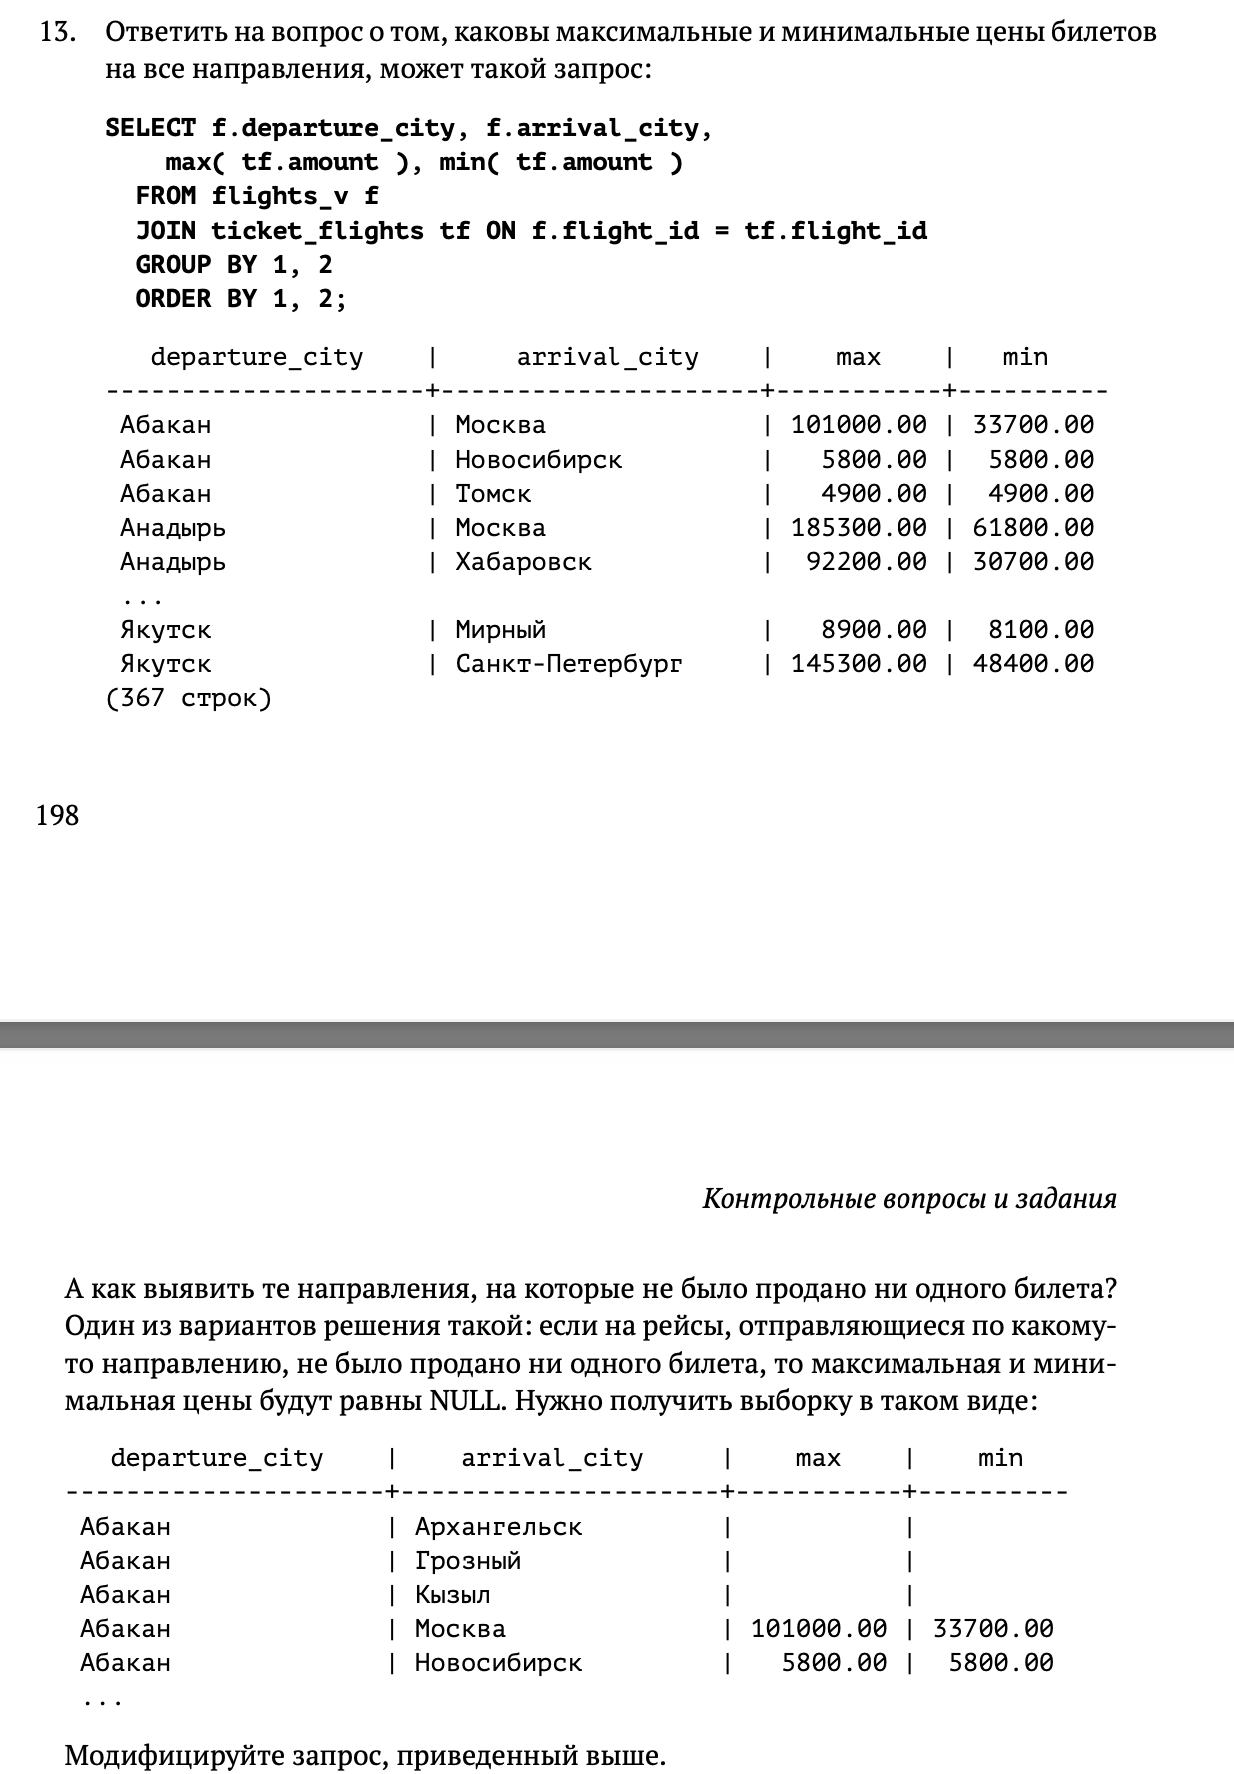
\includegraphics[scale=0.6]{t13.png}
\\\\
\begin{center}
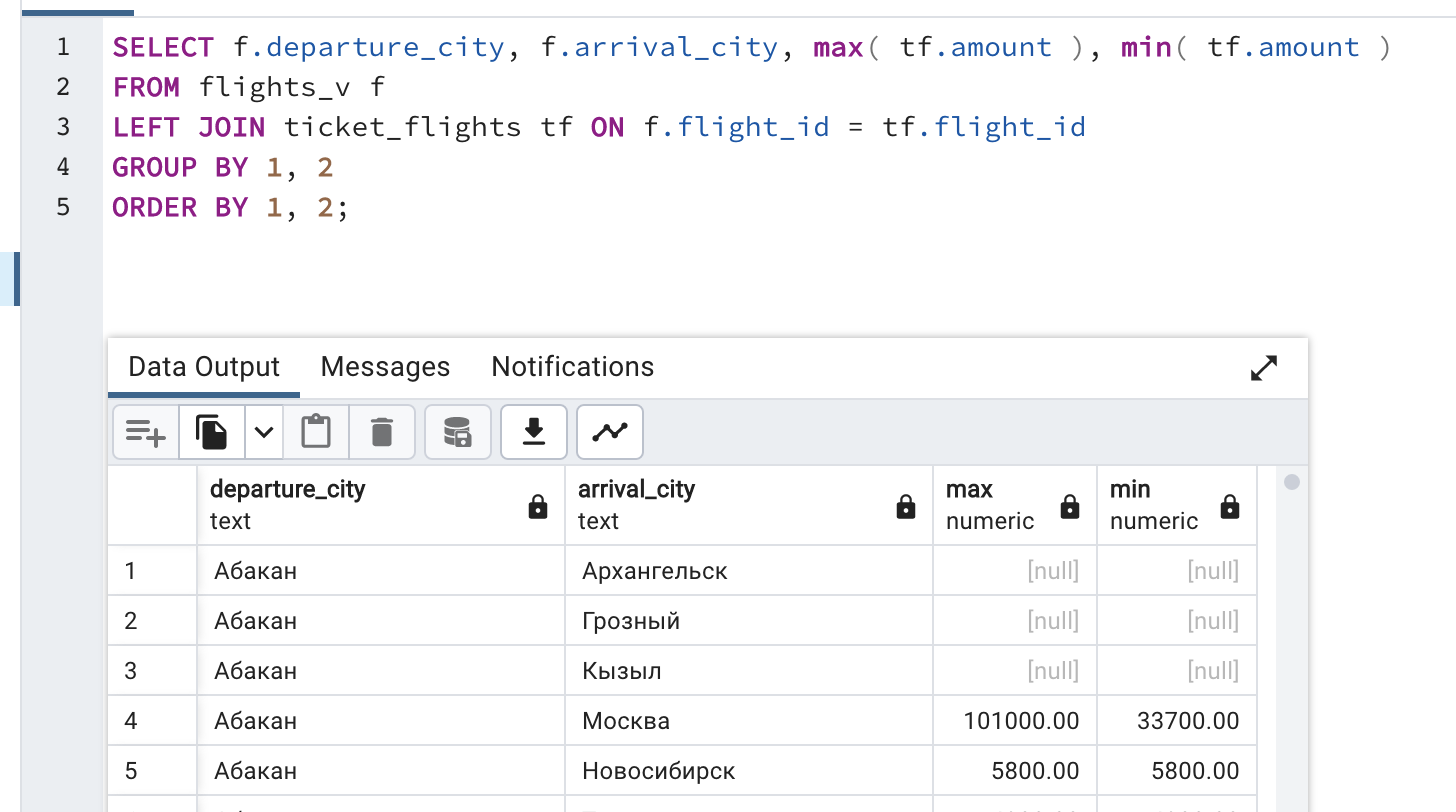
\includegraphics[scale=0.5]{131.png}
\end{center}
\clearpage
\section*{Номер 19}
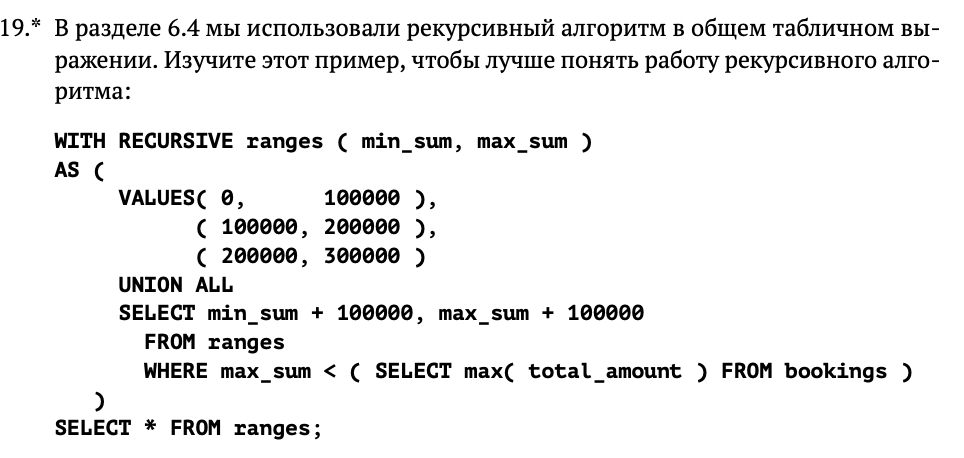
\includegraphics[scale=0.6]{t191.png}
\\\\
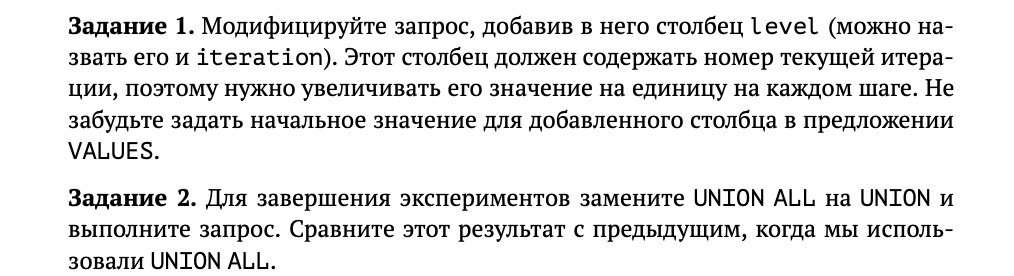
\includegraphics[scale=0.6]{t192.png}
\\\\
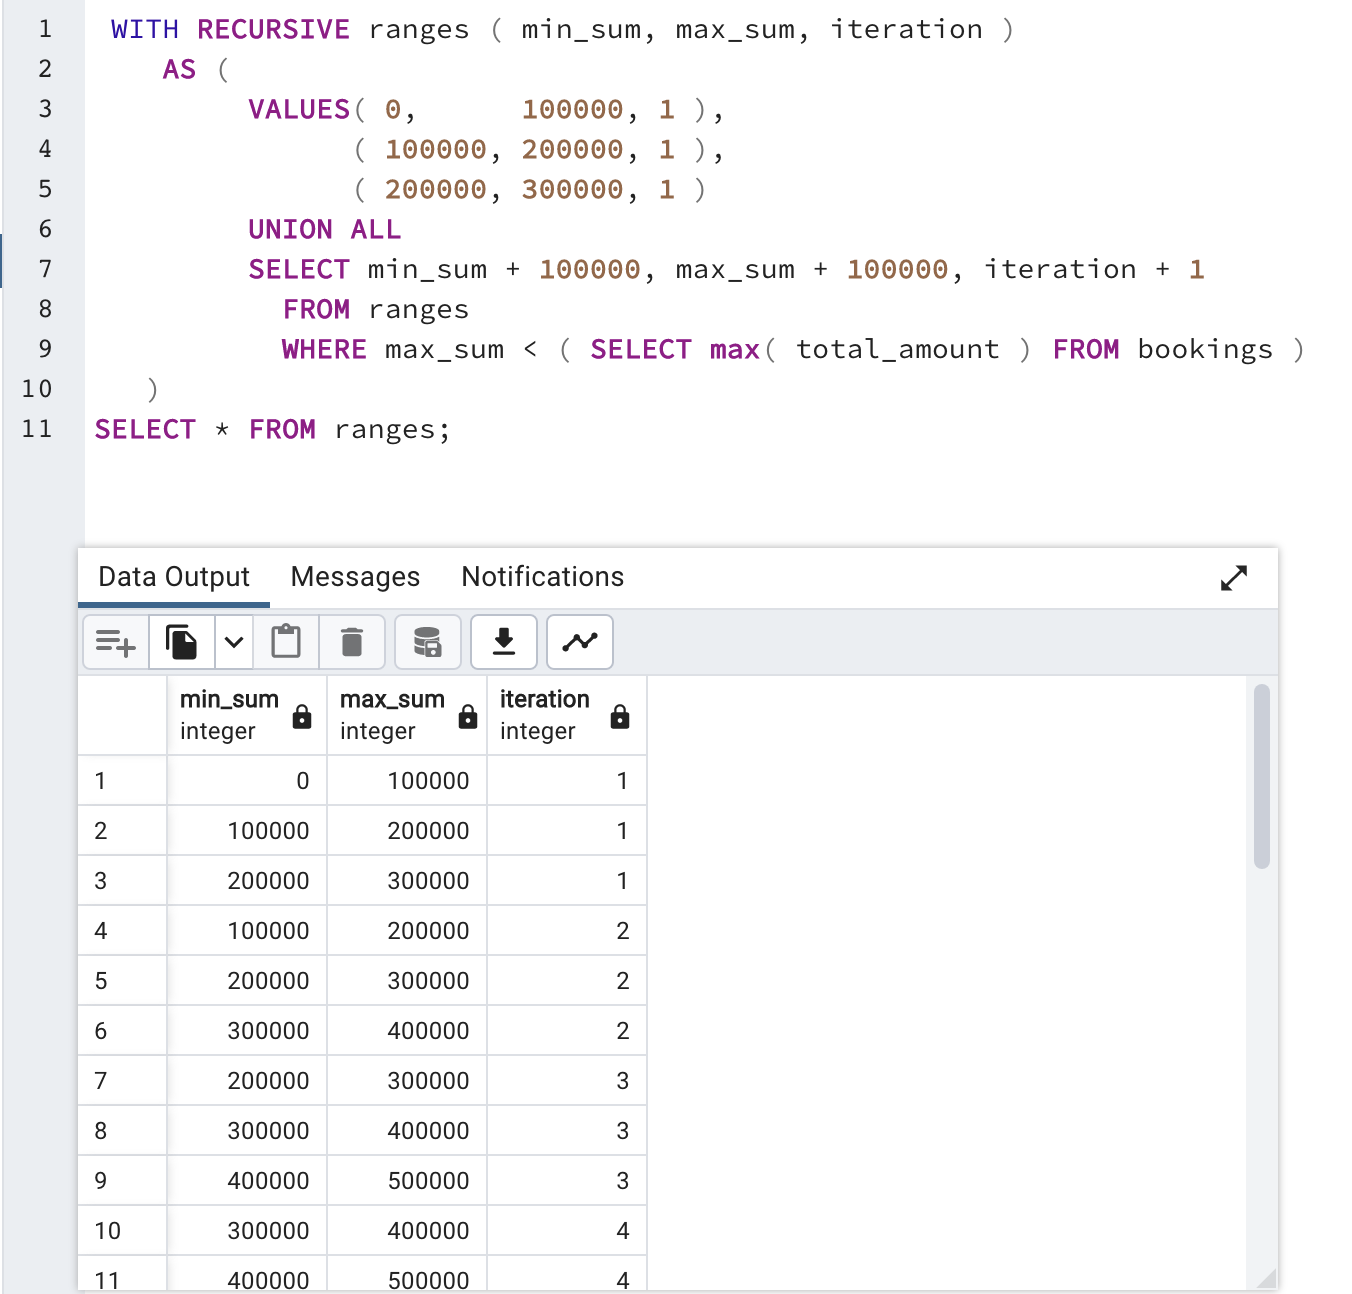
\includegraphics[scale=0.6]{191.png}
\\\\
При замене на UNION удаляются дупликаты, результатом стало уменьшие rows с 36 до 13:
\\
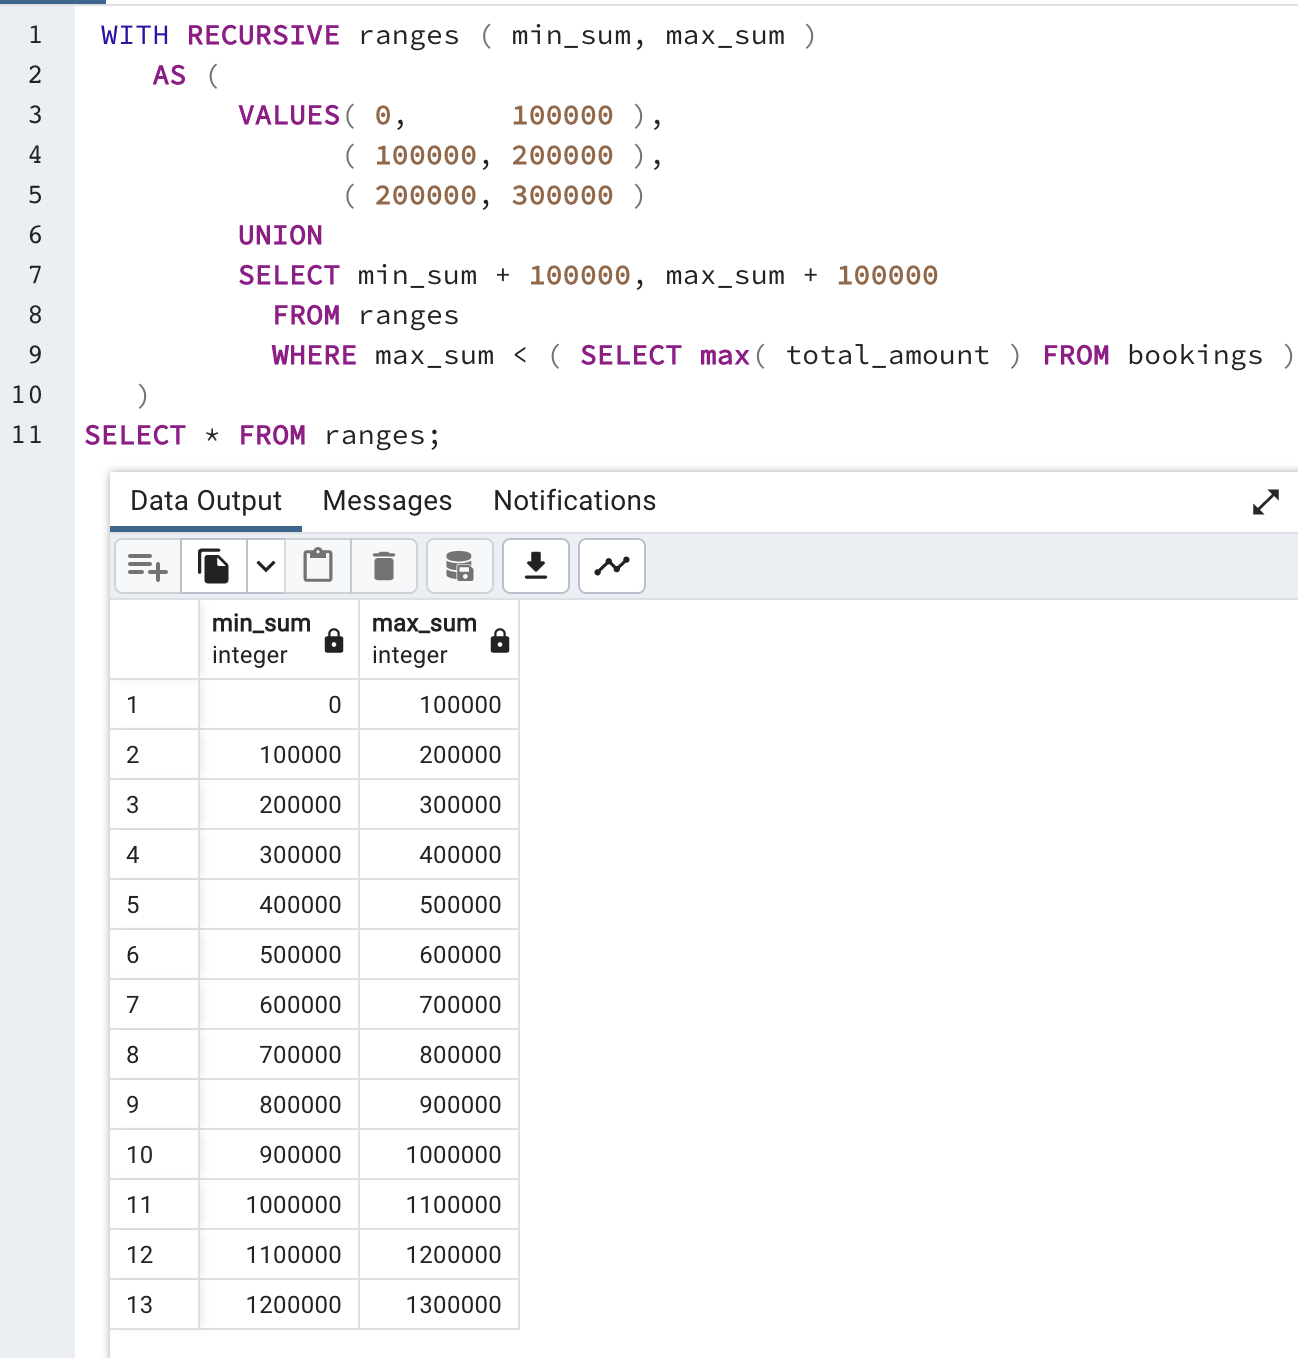
\includegraphics[scale=0.6]{192.png}
\clearpage
\section*{Номер 21}
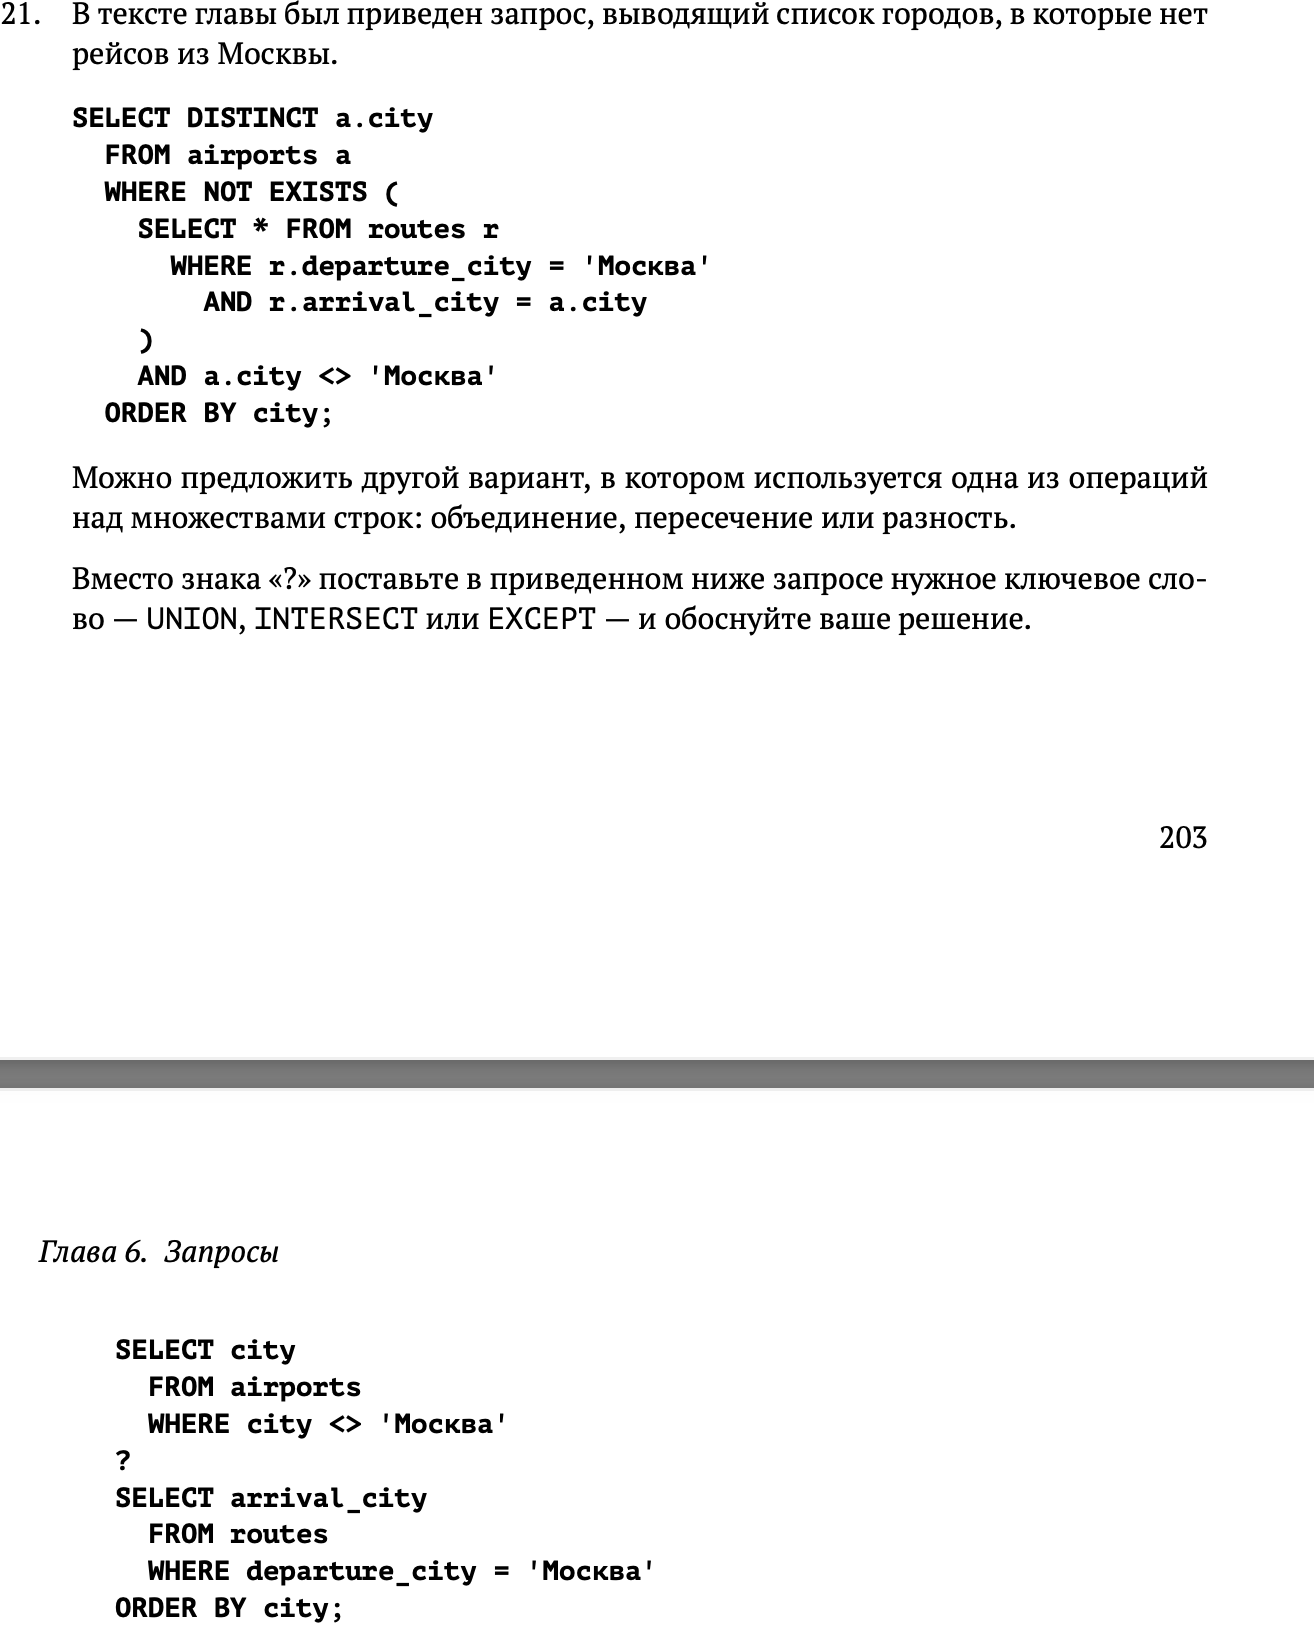
\includegraphics[scale=0.6]{t21.png}
\\\\
\\\\
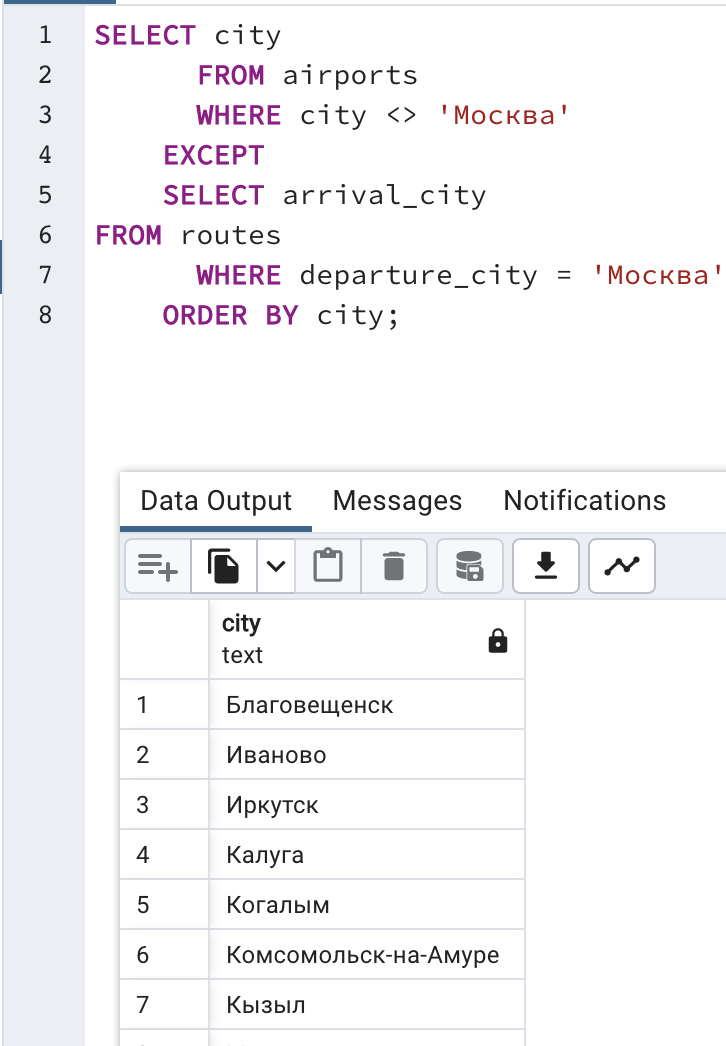
\includegraphics[scale=0.6]{212.png}
\\
Будем использовать EXCEPT, ведь мы хотим исключить оставить все, КРОМЕ Москвы
\clearpage
\section*{Номер 23}
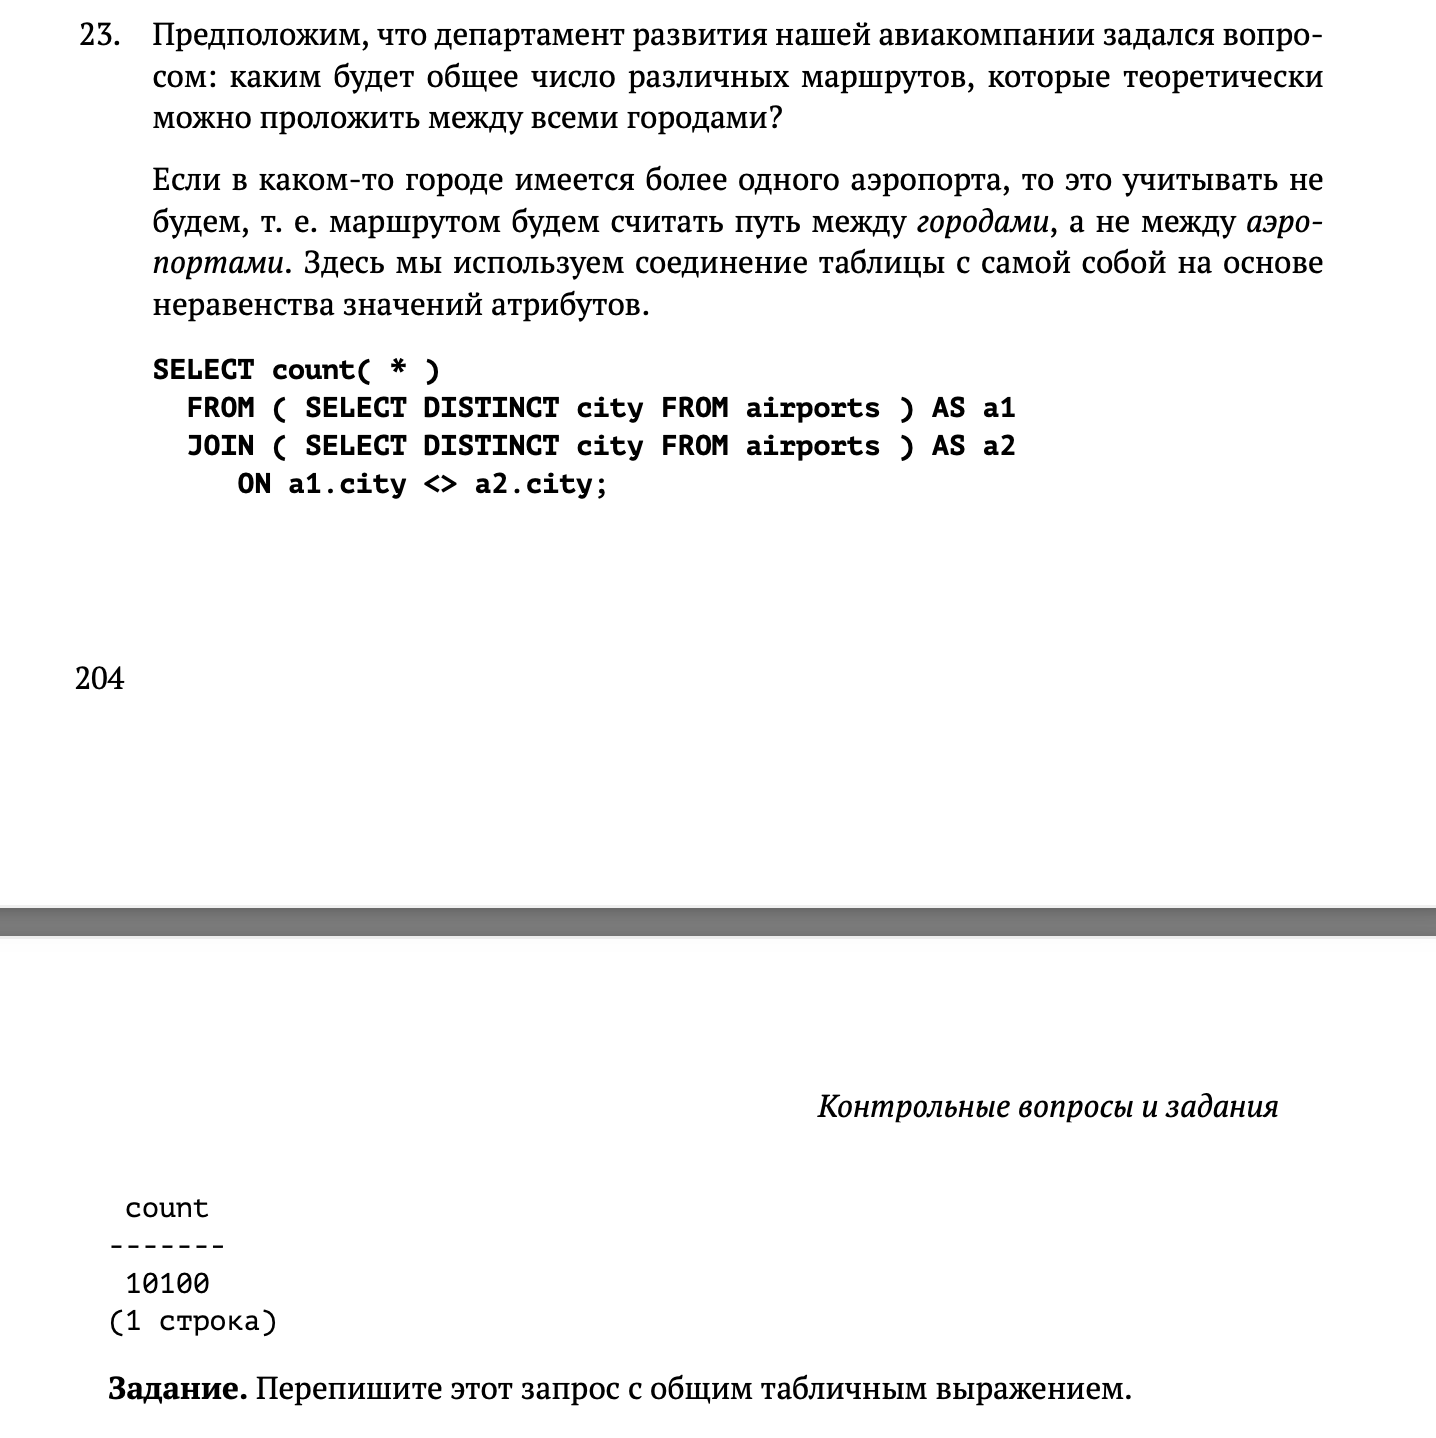
\includegraphics[scale=0.6]{t23.png}
\\\\
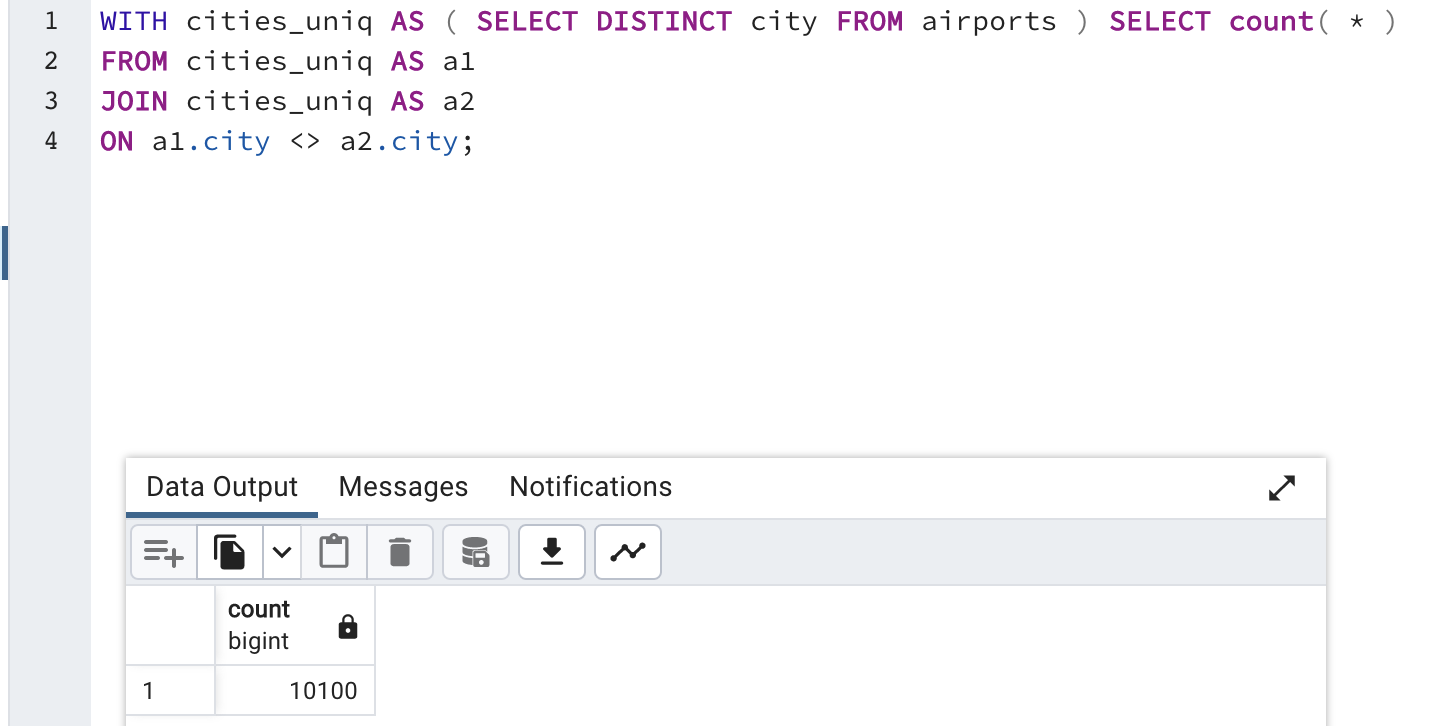
\includegraphics[scale=0.6]{23.png}
\end{document} 
